\section{Proposed Method}\label{sec:method}

%Now comes the ``beef'' of the paper, where you explain what you
%did. Again, organize it in paragraphs with titles. As in every section
%you start with a very brief overview of the section.

%For this class, explain all the optimizations you performed. This mean, you first very briefly
%explain the baseline implementation, then go through locality and other optimizations, and finally SSE (every project will be slightly different of course). Show or mention relevant analysis or assumptions. A few examples: 1) Profiling may lead you to optimize one part first; 2) bandwidth plus data transfer analysis may show that it is memory bound; 3) it may be too hard to implement the algorithm in full generality: make assumptions and state them (e.g., we assume $n$ is divisible by 4; or, we consider only one type of input image); 4) explain how certain data accesses have poor locality. Generally, any type of analysis adds value to your work.
As a baseline we used the libDai library \cite{Mooij_libDAI_10} which provides an implementation for loopy belief propagation using the max residual updating scheme. Using the library is was easy to implement a recommendation system on top of it, closely following \cite{Ha:2012:TRT:2396761.2398636}. One important decision, when dealing with belief propagation, is the one concerning the domain. Switching to a logarithmic domain enables us to express the product over the messages as a sum, often making it less likely to suffer from numerical rounding errors and sometimes making the computation faster. We tested both methods and decided to not utilize the logarithmic domain because the accuracy did not increase and the overhead of transforming the results from/to the log-domain gave us a small increase in the runtime. 

\mypar{Code structure}
Figure \ref{overviewflow} shows a very high level overview of our code structure. After an initialization phase the belief propagation algorithm is invoked. The algorithms then loops until a specified number of maximum iteration is reached, the maximum residual becomes zero or the change in the updated messages is smaller than some specified tolerance. In every iteration 'findMaxResidual' is called to determine the message which should be updated next. After the message is determined it gets updated with a call to 'updateMessage' which also calls 'updateResidual' to update the corresponding residual. This can be done quickly because we already store not only the current messages for each node but also the new message in a container called 'newMessages'. Therefore 'updateMessage' only needs to set the current message to the new one. Finally all messages inside the 'newMessages' container that would be affected by this change needs to be recomputed. We call 'calcNewMessage' which goes through the neighbourhood of the updated message and recomputes the messages, storing the updated version in our 'newMessages' container. In order to compute the new message we first need to compute a product over all incoming messages which is done in 'calcIncomingMessageProduct'. Because we are only interested in a single variable the product is then marginalized (over all other variables) which is done with a call to 'marginalizeProductOntoMessage'. We observe that the methods that get called the most often are 'updateResidual', 'calcIncomingMessageProduct' and 'marginalizeProductOntoMessage'. This is why our optimizations will mostly focus on these.

\begin{figure}\centering
    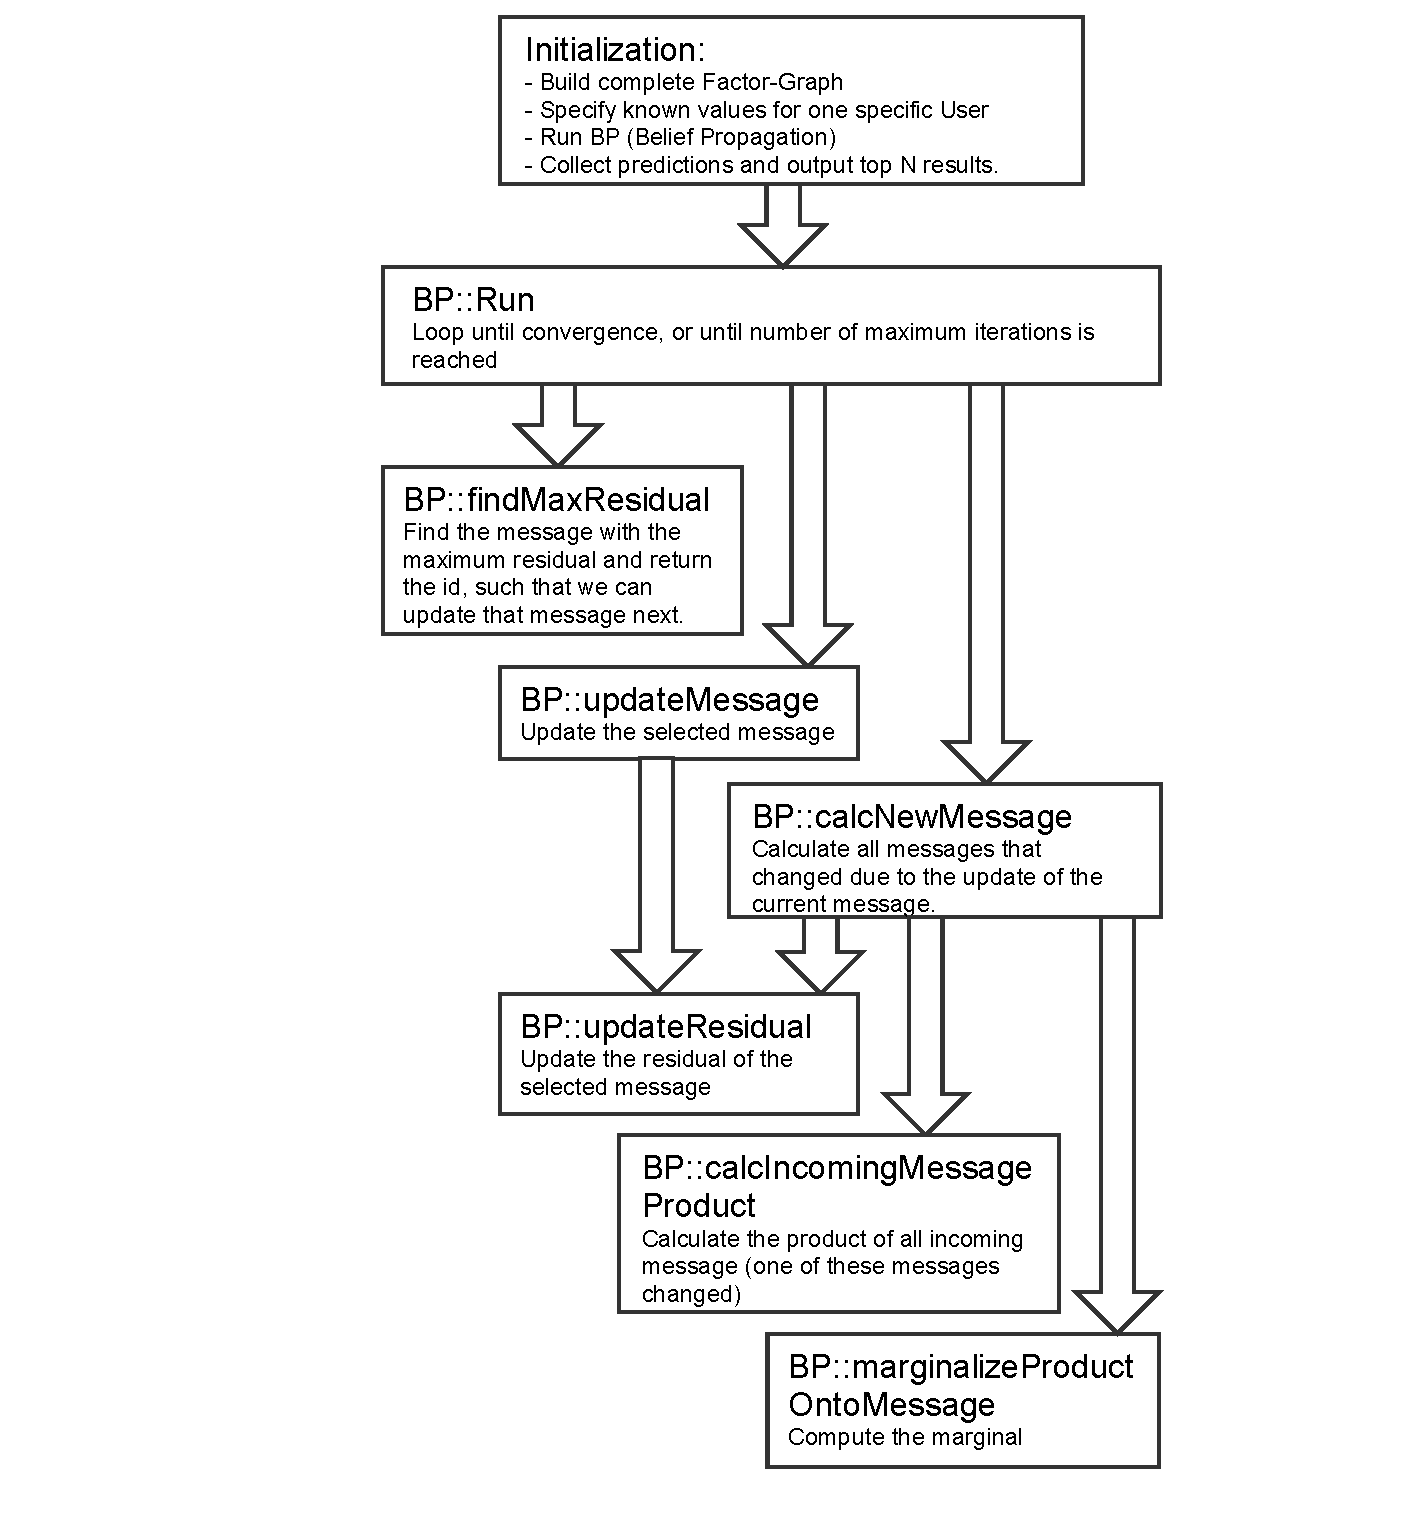
\includegraphics[scale=0.63, trim={6.5cm 0cm 0 0cm},clip]{graphics/loopybp.pdf}
  \caption{Flow (top to bottom) of our program. Arrows denote that a methods gets called from an other, BP is the namespace used for all functions that deal with belief propagation.\label{overviewflow}}
\end{figure}


\mypar{Optimizations}

After we created our baseline and set up a testing environment to automatically validate all our changes we started with the optimizations. We tried to focus on general optimizations first that wouldn't change the interface/functionality of the library. After that was done we focused on our concrete example (recommendation), trading in generality for speed, drastically changing the interface and functionality of the library. In both parts we started with optimizations concerning the number of flops, without considering the computational intensity. We then profiled our code to find critical points where we could optimize memory access patterns or reorder operations to increase the computational intensity. This was also the point where we decided to switch from double to single precision which decreased our accuracy slightly but gave us an significant boost for the runtime. %TODO: How much?
As a final step we considered vectorization which gave us only a very small speed-up. We will know explain all our optimizations in more detail.
 
\mypar{General optimizations}
We started with optimizations that could be applied without changing or limiting the functionality of the library.

The first issue was that we are recomputing the incoming message product every time a message gets updated. This is wasteful because the product could include well over a hundred factors from which only one would change. To avoid the re-computation we compute the product once over all messages. Whenever a message changes we also update the product by multiplying it with the new message and dividing it by the old message. This gave us an speed-up of 1.6 reducing the runtime of the algorithm from 80 to 50 seconds.

Next Norman did a bunch of stuff...

\mypar{Specific optimisations}
Floats -> Double = specific because it changes the result, not okay for a library

Pattern 0101 and 0011

Used the fact that we only stored p, 1-p

Residual

Vectorization
%As important as the final results is to show that you took a structured, organized approach to the optimization and that you explain why you did what you did.

%Mention and cite any external resources including library or other code.

%Good visuals or even brief code snippets to illustrate what you did are good. Pasting large amounts of code to fill the space is not good.
